%%
%% Automatically generated file from DocOnce source
%% (https://github.com/hplgit/doconce/)
%%
%%
% #ifdef PTEX2TEX_EXPLANATION
%%
%% The file follows the ptex2tex extended LaTeX format, see
%% ptex2tex: http://code.google.com/p/ptex2tex/
%%
%% Run
%%      ptex2tex myfile
%% or
%%      doconce ptex2tex myfile
%%
%% to turn myfile.p.tex into an ordinary LaTeX file myfile.tex.
%% (The ptex2tex program: http://code.google.com/p/ptex2tex)
%% Many preprocess options can be added to ptex2tex or doconce ptex2tex
%%
%%      ptex2tex -DMINTED myfile
%%      doconce ptex2tex myfile envir=minted
%%
%% ptex2tex will typeset code environments according to a global or local
%% .ptex2tex.cfg configure file. doconce ptex2tex will typeset code
%% according to options on the command line (just type doconce ptex2tex to
%% see examples). If doconce ptex2tex has envir=minted, it enables the
%% minted style without needing -DMINTED.
% #endif

% #define PREAMBLE

% #ifdef PREAMBLE
%-------------------- begin preamble ----------------------

\documentclass[%
oneside,                 % oneside: electronic viewing, twoside: printing
final,                   % or draft (marks overfull hboxes, figures with paths)
10pt]{article}

\listfiles               % print all files needed to compile this document

\usepackage{relsize,makeidx,color,setspace,amsmath,amsfonts}
\usepackage[table]{xcolor}
\usepackage{bm,microtype}

\usepackage[pdftex]{graphicx}

\usepackage{ptex2tex}
% #ifdef MINTED
\usepackage{minted}
\usemintedstyle{default}
% #endif

\usepackage[T1]{fontenc}
%\usepackage[latin1]{inputenc}
\usepackage{ucs}
\usepackage[utf8x]{inputenc}

\usepackage{lmodern}         % Latin Modern fonts derived from Computer Modern

% Hyperlinks in PDF:
\definecolor{linkcolor}{rgb}{0,0,0.4}
\usepackage{hyperref}
\hypersetup{
    breaklinks=true,
    colorlinks=true,
    linkcolor=linkcolor,
    urlcolor=linkcolor,
    citecolor=black,
    filecolor=black,
    %filecolor=blue,
    pdfmenubar=true,
    pdftoolbar=true,
    bookmarksdepth=3   % Uncomment (and tweak) for PDF bookmarks with more levels than the TOC
    }
%\hyperbaseurl{}   % hyperlinks are relative to this root

\setcounter{tocdepth}{2}  % number chapter, section, subsection

% Tricks for having figures close to where they are defined:
% 1. define less restrictive rules for where to put figures
\setcounter{topnumber}{2}
\setcounter{bottomnumber}{2}
\setcounter{totalnumber}{4}
\renewcommand{\topfraction}{0.85}
\renewcommand{\bottomfraction}{0.85}
\renewcommand{\textfraction}{0.15}
\renewcommand{\floatpagefraction}{0.7}
% 2. ensure all figures are flushed before next section
\usepackage[section]{placeins}
% 3. enable begin{figure}[H] (often leads to ugly pagebreaks)
%\usepackage{float}\restylefloat{figure}

% prevent orhpans and widows
\clubpenalty = 10000
\widowpenalty = 10000

\newenvironment{doconceexercise}{}{}
\newcounter{doconceexercisecounter}
% --- begin definition of \listofexercises command ---
\makeatletter
\newcommand\listofexercises{\section*{List of Exercises and Projects}
\@starttoc{loe}
}
\newcommand*{\l@doconceexercise}{\@dottedtocline{0}{0pt}{6.5em}}
\makeatother
% --- end definition of \listofexercises command ---



% ------ header in subexercises ------
%\newcommand{\subex}[1]{\paragraph{#1}}
%\newcommand{\subex}[1]{\par\vspace{1.7mm}\noindent{\bf #1}\ \ }
\makeatletter
% 1.5ex is the spacing above the header, 0.5em the spacing after subex title
\newcommand\subex{\@startsection{paragraph}{4}{\z@}%
                  {1.5ex\@plus1ex \@minus.2ex}%
                  {-0.5em}%
                  {\normalfont\normalsize\bfseries}}
\makeatother


% --- end of standard preamble for documents ---


% insert custom LaTeX commands...

\raggedbottom
\makeindex

%-------------------- end preamble ----------------------

\begin{document}

% endif for #ifdef PREAMBLE
% #endif


% ------------------- main content ----------------------

% Slides for many-body text


% ----------------- title -------------------------

\thispagestyle{empty}

\begin{center}
{\LARGE\bf
\begin{spacing}{1.25}
Projects and how to develop a numerical project
\end{spacing}
}
\end{center}

% ----------------- author(s) -------------------------

\begin{center}
{\bf Carlo Barbieri, Wim Dickhoff, Gaute Hagen, Morten Hjorth-Jensen, and Artur Polls${}^{}$} \\ [0mm]
\end{center}

\begin{center}
% List of all institutions:
\end{center}
    
% ----------------- end author(s) -------------------------

\begin{center} % date
July 6-24, Ganil, Caen, France
\end{center}

\vspace{1cm}


\tableofcontents


\vspace{1cm} % after toc




\subsection{Plan for the Talent course}
An essential element of the Talent courses is to develop a large project(s) which allows you to study and understand
theoretical concepts in nuclear physics.
These concepts will in turn allow you to interpret results from experiments and understand the pertinent physics in terms of the underlying forces and laws of motion.

Together with the regular lectures in the morning, the hope is that
during these three weeks you will be able to write and run a program
which implements at least one of the methods discussed during the
lectures.  The lectures will also cover additional material which aims
at giving you a broader view on what can be achieved with the methods
to be discussed. Combined with the 'hands-on' afternoon sessions, the
hope is that the lectures and the computational projects will together
allow you to achieve these goals. For those of you who would like to
get credits to be transferred to your home university, the project(s)
can be extended upon allowing you to include further elements to the
many-body methods. The load of the final project is estimated to be
80 hours. In total, attendence at the course and doing
the final project amounts to seven ECTS. There is no credit transfer
for Northern-American students.

\subsection{Outline of the project(s)}

What is outlined here are several paths that will allow you to develop
a program which can be used to study nuclear systems. In particular,
we will focus on two widely used many-body methods, coupled cluster
theory with its various approximations and Green's function theory.

Before we begin, we would however like to present a warm-up problem which
contains
many of the basic elements of the many-body methods exposed in this course. Furthermore, the simple pairing
model described below, provides us with  benchmark results to which we can compare
the different many-body methods. The basic elements of the model (single-particle basis and Hamiltonian)
can easily be (if structured properly in your program) extended to studies of more realistic systems, either
finite systems like nuclei or infinite nuclear matter.

The first part of the project is a traditional paper and pencil part, where the aim is to
apply second quantization in order to set up the Hamiltonian matrix to be diagonalized.
We will study this model the first two afternoons of the school.

At most, with four particles in four doubly degenerate single particle states and no broken pairs,
you will have a $6 \times 6$ Hamiltonian matrix to diagonalize. Below, you will find a simple python program
which performs the diagonalization and plots the eigenvalues. Parts of this warm-up exercise are solved below.
These aspects will be discussed partly during the lectures but also during some of the afternoon sessions.
Practical guidelines for code writing will also be discussed.


This exercise will allow us to start writing our first skeleton for a coupled cluster theory program at the so-called doubles level of truncation. It will also, for those of you who will prefer  to study Green's functions, serve as a
starting point for developing the skeleton of a program for this method. The aim is to finish this part of the program during the first week.

With a program which then benchmarks the simple pairing model, we will turn our attention to more realistic systems.
Here we propose the following  paths that can be studied with either coupled cluster theory or Green's function theory. Many of the technicalities will be discussed at the lectures and the afternoon sessions during the last two weeks.

\begin{enumerate}
\item Studies of nuclear matter with a cartesian basis using coupled cluster theory at the level of doubles excitations
\begin{itemize}

  \item During the three weeks of the course we will mainly focus on two-particle and two-hole excitations

  \item Focusing only on two-particle correlations in a finite cartesian basis, these can be compared with Brueckner-Hartree-Fock calculations in the infinite limit. The latter should represent exactly two-particle correlations to infinite order. A simple model for the nuclear force will be used.

  \item For the final project the code can be extended to include particle-hole correlations as well

\end{itemize}

\noindent
\item The two above paths can be performed using Green's function as well.
\begin{itemize}

  \item Studies of infinite nuclear matter including two-particle and two-hole correlations using a cartesian basis.

  \item Comparison of two-particle correlations from Brueckner-Hartree-Fock calculations in the infinite limit
\end{itemize}

\noindent
\end{enumerate}

\noindent
If there is enough interest, we can also develop projects where Coupled Cluster theory and Green's function theories are applied to finite systems. In this case we would like to propose a simple system of neutrons in a harmonic oscillator trap since these calculations can be benchmarked agains \href{{http://journals.aps.org/prc/abstract/10.1103/PhysRevC.84.044306}}{existing results}.


When working on the projects, we recommend strongly that you form teams of two to three participants. Every team
\textbf{must} have a \emph{github account} where we can monitor your progress and give you appropriate feedback.

If you have not used version control before now, it is time to do so.
Proper version control is central to a good ethical scientific conduct.
We do require that you use some kind of version control software when working on the projects. We recommend strongly \href{{https://github.com/}}{github}. All lectures and additional material is available at the github \href{{http://nucleartalent.github.io/Course2ManyBodyMethods/doc/web/course.html}}{address of the course}

Furthermore, before coming to the course, we recommend that you refresh your knowledge on second quantization.
If your background in second quantization is rudimentary and mentioning of Wick's leave you gazing at the stars,
we recommend that you study the material at the course web site on \href{{http://nucleartalent.github.io/Course2ManyBodyMethods/doc/pub/secondquant/html/secondquant-bs.html}}{second quantization}. Try in particular to do some of the exercises.

We will also ask  you to come with your own laptop and have installed either a
\begin{itemize}
\item Fortran compiler or a

\item c++ compiler
\end{itemize}

\noindent
If you do not have your own laptop, there will be some PCs locally with the relevant compilers and software.

You can use Python as programming language as well, but normally the efficiency of Python for the problems addressed in this course is lower than for codes written in Fortran or c++. We recommend however that use Python as a scripting language for running codes and making plots, as well as using the ipython notebooks provided by us.

\subsection{Some basic ingredients for a successful numerical project}

When building up a numerical project there are several elements you should think of, amongst these we take the liberty of mentioning the following:
\begin{enumerate}
  \item How to structure a code in terms of functions

  \item How to make a module

  \item How to read input data flexibly from the command line

  \item How to create graphical/web user interfaces

  \item How to write unit tests (test functions)

  \item How to refactor code in terms of classes (instead of functions only), in our case you think of a system and a solver class

  \item How to conduct and automate large-scale numerical experiments

  \item How to write scientific reports in various formats ({\LaTeX}, HTML)
\end{enumerate}

\noindent
The conventions and techniques outlined here will save you a lot of time when you incrementally extend software over time from simpler to more complicated problems. In particular, you will benefit from many good habits:
\begin{enumerate}
\item New code is added in a modular fashion to a library (modules)

\item Programs are run through convenient user interfaces

\item It takes one quick command to let all your code undergo heavy testing

\item Tedious manual work with running programs is automated,

\item Your scientific investigations are reproducible, scientific reports with top quality typesetting are produced both for paper and electronic devices.
\end{enumerate}

\noindent
\subsection{The pairing model as warm-up problem}

We present a simplified Hamiltonian consisting of an unperturbed
Hamiltonian and a so-called pairing interaction term. It is a model
which to a large extent mimicks some central features of atomic
nuclei, certain atoms and systems which exhibit superfluiditity or
superconductivity.  To study this system, we will use a mix of
many-body perturbation theory (MBPT), Hartree-Fock (HF) theory and full
configuration interaction (FCI) theory. The latter will also provide us with
the exact answer.  When setting up the Hamiltonian matrix you will
need to solve an eigenvalue problem.

We define first the Hamiltonian, with a definition of the model space
and the single-particle basis. Thereafter, we present the various
exercises (some of them are solved).


The Hamiltonian acting in the complete Hilbert space (usually infinite
dimensional) consists of an unperturbed one-body part, $\hat{H}_0$,
and a perturbation $\hat{V}$.

We limit ourselves to at most two-body interactions and our Hamiltonian
is represented by the following operators
\[
\hat{H} = \sum_{\alpha\beta}\langle \alpha |h_0|\beta\rangle
a_{\alpha}^{\dagger}a_{\beta}+\frac{1}{4}\sum_{\alpha\beta\gamma\delta}\langle \alpha\beta|
V|\gamma\delta\rangle a_{\alpha}^{\dagger}a_{\beta}^{\dagger}a_{\delta}a_{\gamma},
\]
where $a_{\alpha}^{\dagger}$ and $a_{\alpha}$ etc.~are standard
fermion creation and annihilation operators, respectively, and
$\alpha\beta\gamma\delta$ represent all possible single-particle
quantum numbers.  The full single-particle space is defined by the
completeness relation
\[
\hat{{\bf 1}} = \sum_{\alpha=1}^{\infty}|\alpha \rangle \langle \alpha|.
\]
In our calculations
we will let the single-particle states $|\alpha\rangle$ be
eigenfunctions of the one-particle operator $\hat{h}_0$. Note that the two-body part of the Hamiltonian
contains anti-symmetrized matrix elements.


The above Hamiltonian acts in turn on various many-body Slater
determinants constructed from the single-basis defined by the one-body
operator $\hat{h}_0$.  As an example, the two-particle model space
$\mathcal{P}$ is defined by an operator
\[
\hat{P} = \sum_{\alpha\beta =1}^{m}|\alpha\beta \rangle \langle
\alpha\beta|,
\]
where we assume that $m=\dim(\mathcal{P})$ and the full space is
defined by
\[
\hat{P}+\hat{Q}=\hat{{\bf 1}},
\]
with the projection operator
\[
\hat{Q} = \sum_{\alpha\beta =m+1}^{\infty}|\alpha\beta \rangle \langle
\alpha\beta|,
\]
being the complement of $\hat{P}$.


Our specific model consists of $N$ doubly-degenerate and equally
spaced single-particle levels labelled by $p=1,2,\dots$ and spin
$\sigma=\pm 1$.  These states are schematically portrayed in
Fig.~\ref{fig:schematic}.  The first two single-particle levels define
a possible model space, indicated by the label $\mathcal{P}$.  The
remaining states span the excluded space $\mathcal{Q}$.

We write the Hamiltonian as
\[ \hat{H} = \hat{H}_0 + \hat{V} , \]
where
\[
\hat{H}_0=\xi\sum_{p\sigma}(p-1)a_{p\sigma}^{\dagger}a_{p\sigma}
\]
and
\[
\hat{V}=-\frac{1}{2}g\sum_{pq}a^{\dagger}_{p+}
a^{\dagger}_{p-}a_{q-}a_{q+}.
\]
Here, $H_0$ is the unperturbed Hamiltonian with a spacing between
successive single-particle states given by $\xi$, which we will set to
a constant value $\xi=1$ without loss of generality. The two-body
operator $\hat{V}$ has one term only. It represents the pairing
contribution and carries a constant strength $g$.

The indices
$\sigma=\pm$ represent the two possible spin values. The interaction
can only couple pairs and excites therefore only two particles at the
time, as indicated by the rightmost four-particle state in
Fig.~\ref{fig:schematic}. There one of the pairs is excited to the
state with $p=9$ and the other to the state $p=7$. The two middle
possibilities are not possible with the present model.  We label
single-particle states within the model space as hole-states. The
single-particle states outside the model space are then particle
states.

In our model we have kept both the interaction strength and the
single-particle level as constants.  In a realistic system like an
atom or the atomic nucleus this is not the case.


\begin{figure}[t]
  \centerline{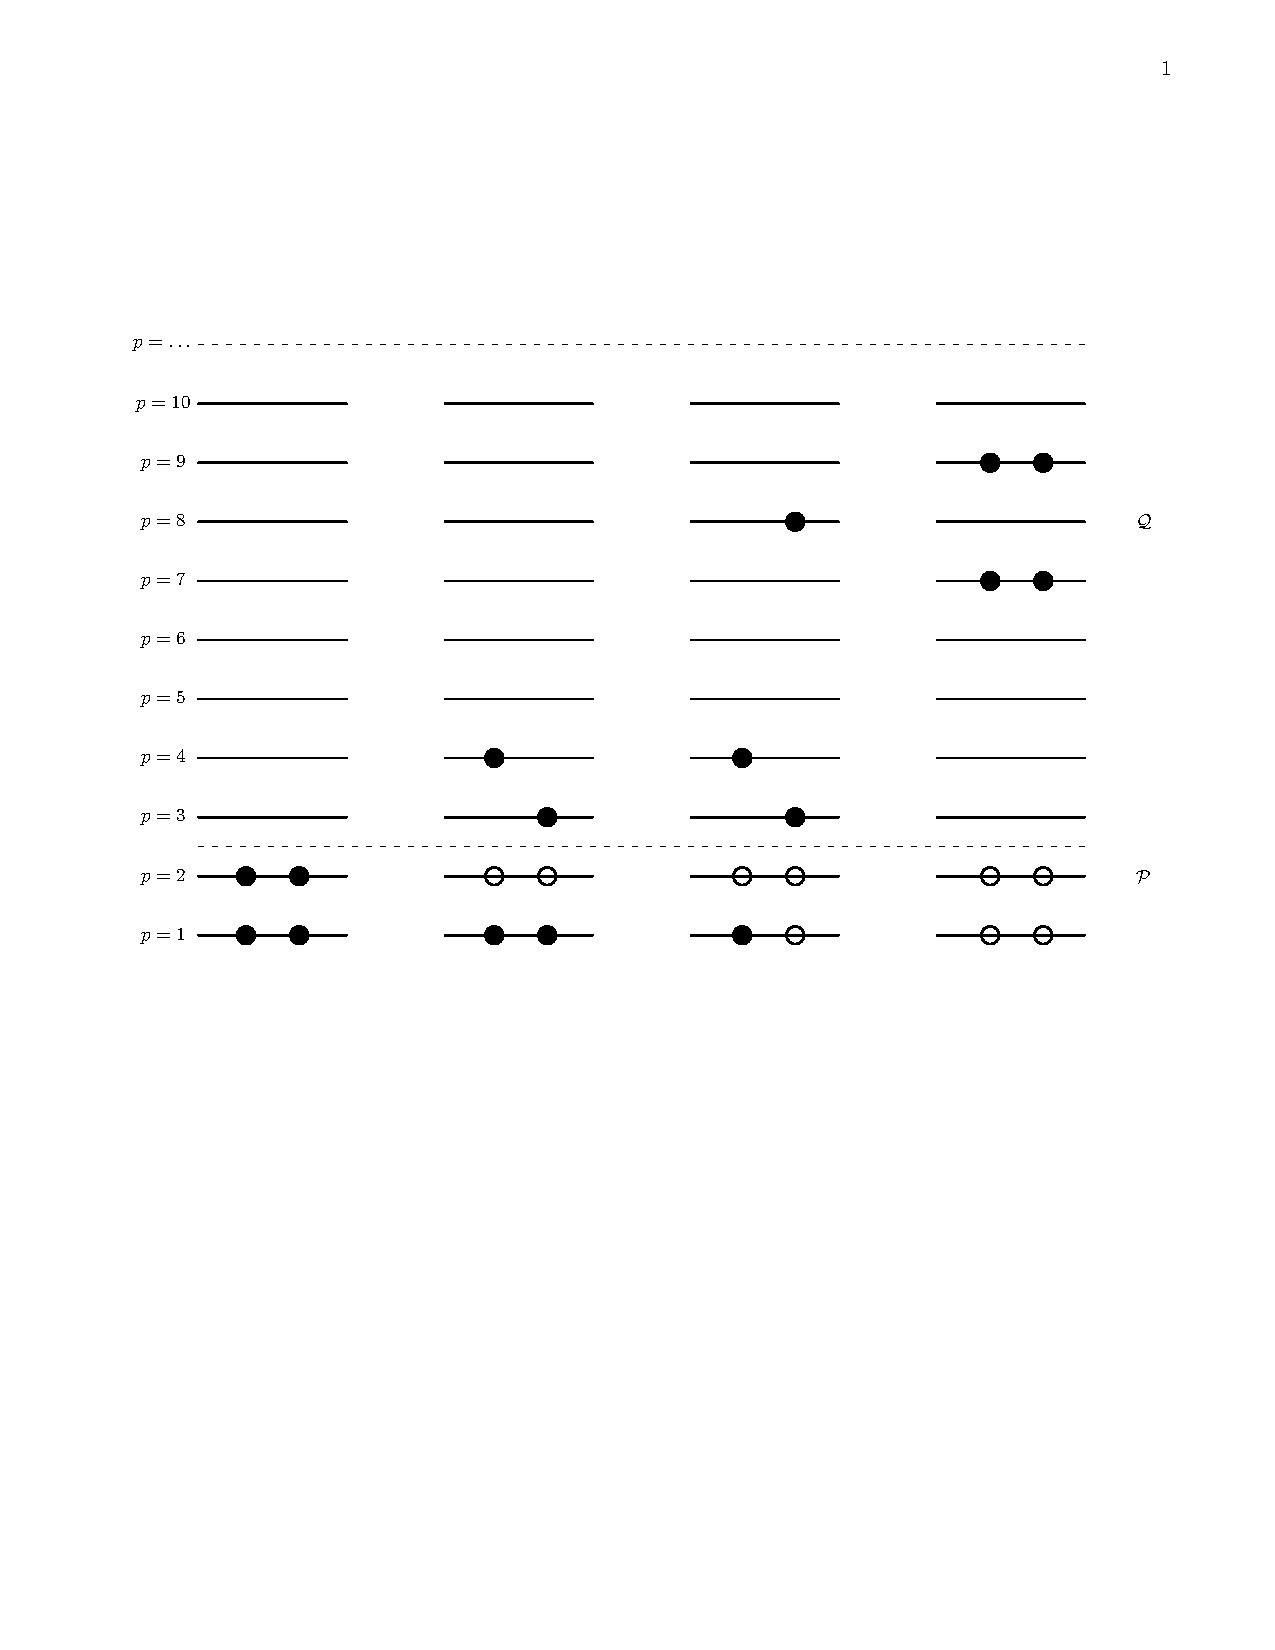
\includegraphics[width=0.7\linewidth]{fig-proj/simplemodel.pdf}}
  \caption{
  Schematic plot of the possible single-particle levels with double degeneracy.  The filled circles indicate occupied particle  states while the empty circles represent vacant particle(hole)  states.  The spacing between each level $p$ is constant in this picture.  The first two single-particle levels define our possible  model space, indicated by the label $\mathcal{P}$.  The remaining  states span the excluded space $\mathcal{Q}$.  The first state to  the left represents a possible ground state representation for a  four-fermion system. In the second state to the left, one pair is   broken. This possibility is however not included in our  interaction. \label{fig:schematic}
  }
\end{figure}
%\clearpage % flush figures fig:schematic




% --- begin exercise ---
\begin{doconceexercise}
\refstepcounter{doconceexercisecounter}

\subsection*{Exercise \thedoconceexercisecounter: Pairing Hamiltonian}



\subex{a)}
Show that the unperturbed Hamiltonian $\hat{H}_0$ and $\hat{V}$
  commute with both the spin projection $\hat{S}_z$ and the total spin
  $\hat{S}^2$, given by
\[
  \hat{S}_z := \frac{1}{2}\sum_{p\sigma} \sigma
  a^{\dagger}_{p\sigma}a_{p\sigma}
\]
and
\[
  \hat{S}^2 := \hat{S}_z^2 + \frac{1}{2}(\hat{S}_+\hat{S}_- +
  \hat{S}_-\hat{S}_+),
\]
where
\[
  \hat{S}_\pm := \sum_{p} a^{\dagger}_{p\pm} a_{p\mp}.
\]
This is an important feature of our system that allows us to
block-diagonalize the full Hamiltonian. We will focus on total spin
$S=0$.  In this case, it is convenient to define the so-called pair
creation and pair annihilation operators
\[
\hat{P}^{+}_p = a^{\dagger}_{p+}a^{\dagger}_{p-},
\]
and
\[
\hat{P}^{-}_p = a_{p-}a_{p+},
\]
respectively.

Show that you can rewrite the Hamiltonian (with $\xi=1$) as
\[
\hat{H}=\sum_{p\sigma}(p-1)a_{p\sigma}^{\dagger}a_{p\sigma}
-\frac{1}{2}g\sum_{pq}\hat{P}^{+}_p\hat{P}^{-}_q.
\]
Show also that Hamiltonian commutes with the product of the pair
creation and annihilation operators.  This model corresponds to a
system with no broken pairs. This means that the Hamiltonian can only
link two-particle states in so-called spin-reversed states.


\subex{b)}
Construct thereafter the Hamiltonian matrix for a system with no
  broken pairs and total spin $S=0$ for the case of the four lowest
  single-particle levels indicated in the
  Fig.~\ref{fig:schematic}. Our system consists of four particles
  only.  Our single-particle space consists of only the four lowest
  levels $p=1,2,3,4$.  You need to set up all possible Slater
  determinants.  Find all eigenvalues by diagonalizing the Hamiltonian
  matrix.  Vary your results for values of $g\in [-1,1]$.  We refer to
  this as the exact calculation. Comment the behavior of the ground
  state as function of $g$.


% --- begin solution of exercise ---
\paragraph{Solution.}
We give first the final Hamiltonian matrix
\[
H = \left (
\begin{array}{cccccc}
2\delta -g & -g/2 & -g/2 & -g/2 & -g/2 & 0 \\
 -g/2 & 4\delta -g & -g/2 & -g/2 & -0 & -g/2 \\
-g/2 & -g/2 & 6\delta -g & 0 & -g/2 & -g/2 \\
 -g/2 & -g/2 & 0 & 6\delta-g & -g/2 & -g/2 \\
 -g/2 & 0 & -g/2 & -g/2 & 8\delta-g & -g/2 \\
0 & -g/2 & -g/2 & -g/2 & -g/2 & 10\delta -g
\end{array} \right )
\]
The following python program diagonalizes the above Hamiltonian matrix for a given span of interaction strength values, performing both a full configuration interaction calculation and a truncated one. For the truncated case we leave out the $4p4h$ state. This means that in addition to the ground state we include the four possible $2p2h$ states. Such a calculation is normally called a configuration interaction calculation.
\bpypro
from numpy import *
from sympy import *
from matplotlib.pyplot import *

g_array = linspace(-1, 1, 1001)
e1_array = []
e2_array = []

for g in g_array:
	H1 = matrix([[2-g , -g/2.,  -g/2., -g/2., -g/2.,     0],
		        [-g/2.,   4-g,  -g/2., -g/2.,    0., -g/2.],
		        [-g/2., -g/2.,    6-g,     0, -g/2., -g/2.],
				[-g/2., -g/2.,      0,   6-g, -g/2., -g/2.],
				[-g/2.,     0,  -g/2., -g/2.,   8-g, -g/2.],
				[0    , -g/2.,  -g/2., -g/2., -g/2.,  10-g]])

	H2 = matrix([[2-g , -g/2.,  -g/2., -g/2., -g/2.],
		        [-g/2.,   4-g,  -g/2., -g/2.,    0.],
		        [-g/2., -g/2.,    6-g,     0, -g/2.],
				[-g/2., -g/2.,      0,   6-g, -g/2.],
				[-g/2.,     0,  -g/2., -g/2.,   8-g]])



	u1, v1 = linalg.eig(H1)
	u2, v2 = linalg.eig(H2)

	if g == 1./2:
		print argmin(u1)

		for i in range(5):
			print " %.3f " % v2[i,0],



	e1_array.append(min(u1))
	e2_array.append(min(u2))


plot(g_array, e1_array, linewidth=2.0)
#plot(g_array, e2_array, linewidth=2.0)
plot(g_array, (2-g_array), linewidth=2.0)
grid()
xlabel(r"Strength of interaction, $g$", fontsize=16)
ylabel(r'Ground state energy', fontsize=16)
#axis([-1,1,-0.4,0.05])
legend(['FCI -- Exact', 'Reference energy'])
savefig("pairing.pdf")
show()
\epypro
The eigenvalues and eigenvectors result from the diagonalization of the above Hamiltonian matrix.
In the discussions below and in connection with the first stage of the numerical project, we will use these results to benchmark various approximative methods.
The lowest eigenvalue corresponds to the ground state
energy and we will refer to it as the \emph{exact energy} when no truncations in the space of possible Slater determinants are made..

From our results, we note some important differences between the full configuration interaction (FCI)
calculation and the truncated configuration interaction calculation (CI).
Full configuration interaction is an exact method, but is only
possible if and only if we have a complete and finite SD basis for our
system. In practice, we usually don't have this. Non-complete
CI however, is always possible, but yiels   approximative
results only. The method is however still variational however, meaning that we
guaranteed that the approximation will be equal or bigger to the true
result.
Perturbation theory however, is non-variational and there is no guarantee that including higher orders in the
perturbation gives an improved result, as we will see below.

In an FCI case, we are including all possible exictations to infinite
order, meaning we have all possible $1p1h$ , $2p2h$ etc configurations, up to $4p4h$
excitations for our selected model. Due to the nature of the pairing interaction and our selection
of specific quantum numbers for the many-body states, we do not have any $1p1h$ or $3p3h$ excitations.
In the above CI case, we truncate those excitations somewhere.
If we
were to draw the diagrams of the interactions that contribute to this
CI case, there would be an infinite number of them, as we can have
arbitrarily long chains of operators that still only have at most 2p2h
intermediate states.

% --- end solution of exercise ---

\subex{c)}
We switch now to approximative methods, in our case Hartree-Fock
  theory and many-body perturbation theory. Hereafter we will define
  our model space to consist of the single-particle levels $p=1,2$.
  The remaining levels $p=3,4$ define our excluded space.  This means
  that our ground state Slater determinant consists of four particles
  which can be placed in the doubly degenerate orbits $p=1$ and $p=2$.
  Our first step is to perform a Hartree-Fock calculation with the
  pairing Hamiltonian.  Write first the normal-ordered Hamiltonian
  with respect to the above reference state given by four spin $1/2$
  fermions in the single-particle levels $p=1,2$. Define what is meant
  by a canonical Hartree-Fock case, a non-canonical case and a general
  case.  For all three cases, write down the normal-ordered
  Hamiltonian and draw the diagrammatic form of the Hamiltonian for all three cases.



\subex{d)}
We will now set up the Hartree-Fock equations by varying the
coefficients of the single-particle functions. The single-particle
basis functions are defined as
\[
\psi_p = \sum_{\lambda} C_{p\lambda}\psi_{\lambda}.
\]
where in our case $p=1,2,3,4$ and $\lambda=1,2,3,4$, that is the first
four lowest single-particle orbits of Fig.~\ref{fig:schematic}.  Set
up the Hartree-Fock equations for this system by varying the
coefficients $C_{p\lambda}$ and solve them for values of $g\in
[-1,1]$.  Comment your results and compare with the exact
solution. Discuss also which diagrams in Fig.~\ref{fig:diagrams} that
can be affected by a Hartree-Fock basis. Compute the total binding
energy using a Hartree-Fock basis and comment your results.



\subex{e)}
We will now study the system using non-degenerate
Rayleigh-Schroedinger perturbation theory to third order in the
interaction.  If we exclude the first order contribution, all possible
diagrams (so-called anti-symmetric Goldstone diagrams) are
shown in Fig.~\ref{fig:diagrams}.


\begin{figure}[t]
  \centerline{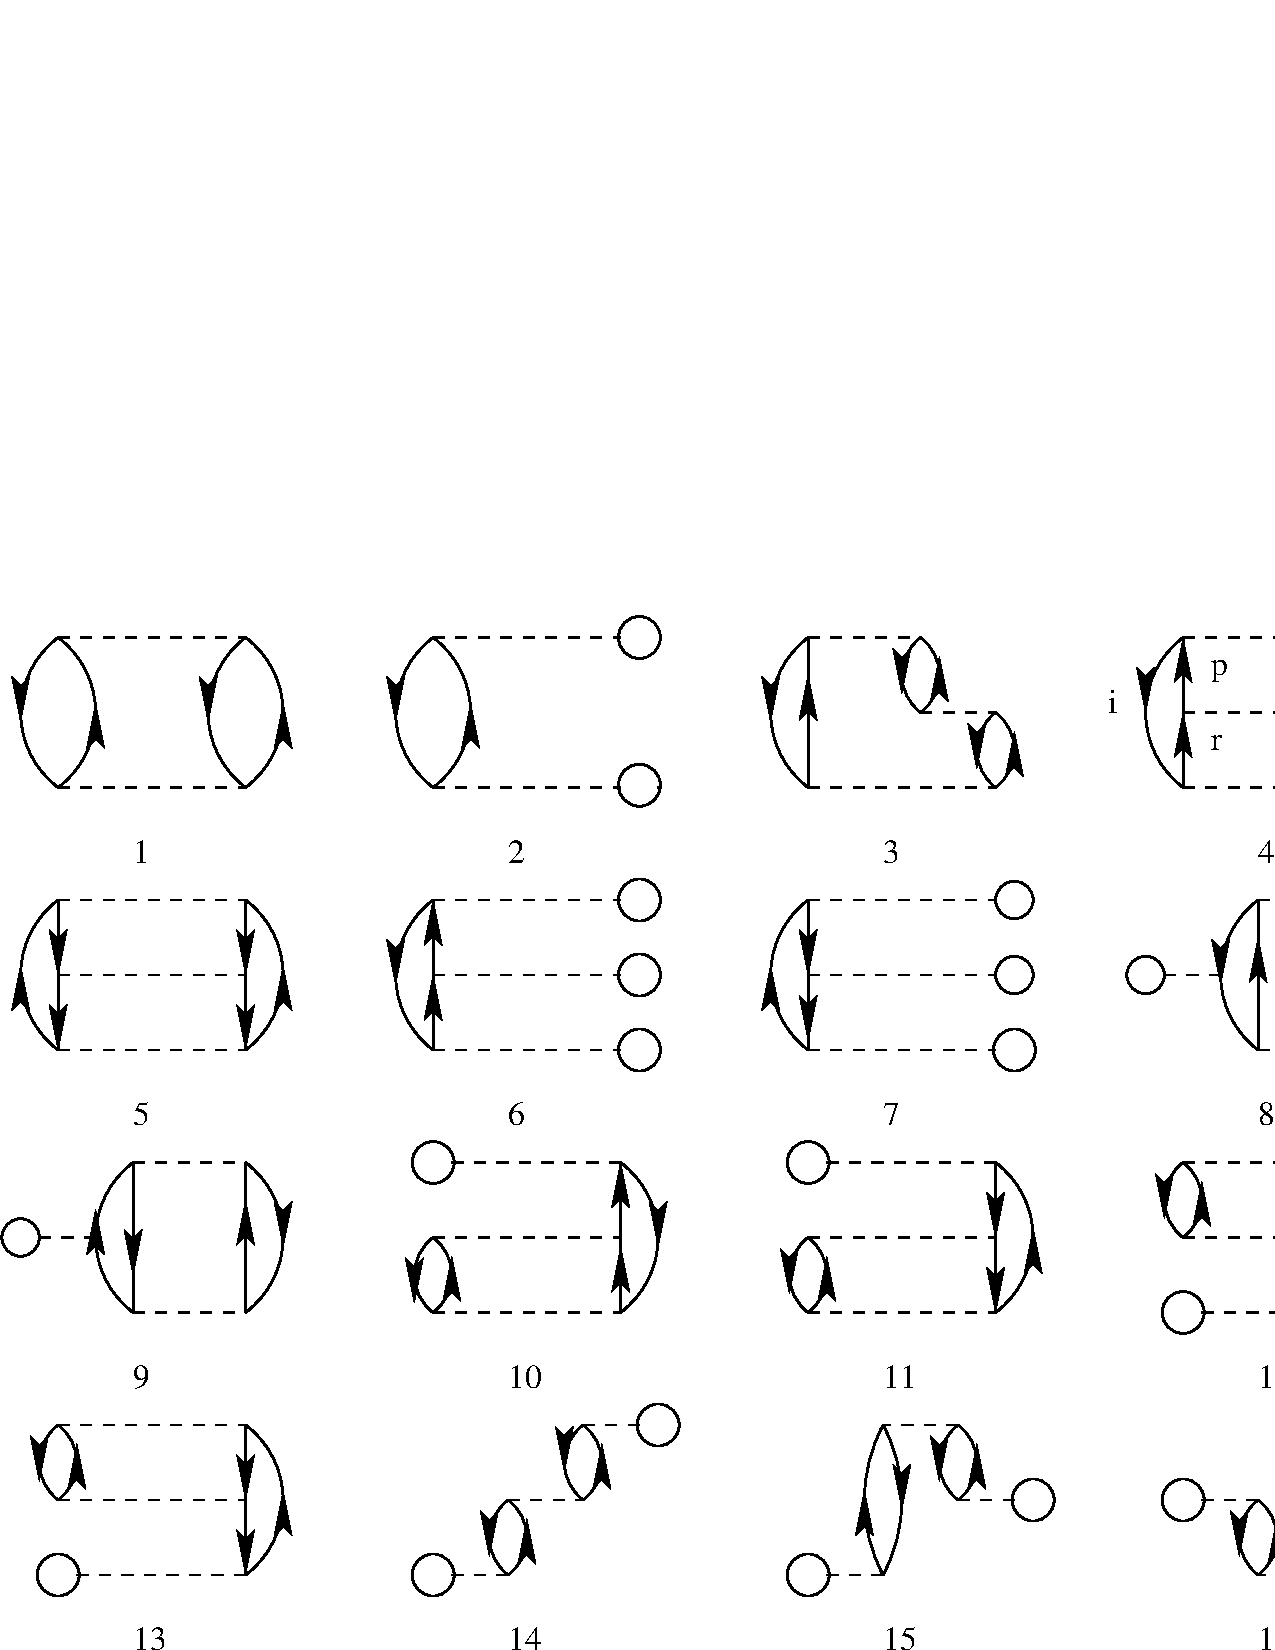
\includegraphics[width=0.6\linewidth]{fig-proj/diagrams.pdf}}
  \caption{
  Diagrams to third order in the interaction, including also non-canonical Hartree-Fock diagrams. The first order term is excluded. All interaction vertices represent anti-symmetrized matrix elements. \label{fig:diagrams}
  }
\end{figure}
%\clearpage % flush figures fig:diagrams


Based on the form of the interaction, which diagrams contribute to the
binding energy of the ground state?  Write down the expressions for
the diagrams that contribute and find the contribution to the ground
state energy as function $g\in [-1,1]$. Comment your results.  Compare
these results with those you obtained from the exact diagonalization with and without the $4p-4h$ state.
Discuss your results for a canonical Hartree-Fock basis and a non-canonical Hartree-Fock basis.

\subex{f)}
Diagram 1 in Fig.~\ref{fig:diagrams} represents a second-order contribution to the energy and a so-called $2p-2h$ contribution to the intermediate states. Write down the expression for the wave operator in this case and compare the possible contributions with the configuration interaction calculations without the $4p-4h$ Slater determinant. Comment your results for
various values of $g\in [-1,1]$.

\subex{g)}
We limit now the discussion to the canonical Hartree-Fock case only. To fourth order in perturbation theory we can produce diagrams with $1p-1h$ intermediate excitations as shown in Fig.~\ref{fig:fourthorder1p1h}, $2p-2h$ excitations, see Fig.~\ref{fig:fourthorder2p2h}, $3p-3h$ excitations as shown in Fig.~\ref{fig:fourthorder3p3h} and finally so-called diagrams with intermediate four-particle-four-hole excitations, see Fig.~\ref{fig:fourthorder4p4h}.


\begin{figure}[t]
  \centerline{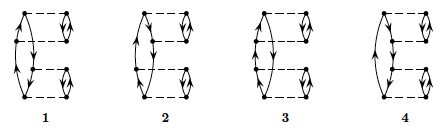
\includegraphics[width=0.6\linewidth]{fig-proj/fourthorder1p1h.png}}
  \caption{
  One-particle-one-hole excitations to fourth order. \label{fig:fourthorder1p1h}
  }
\end{figure}
%\clearpage % flush figures fig:fourthorder1p1h



\begin{figure}[t]
  \centerline{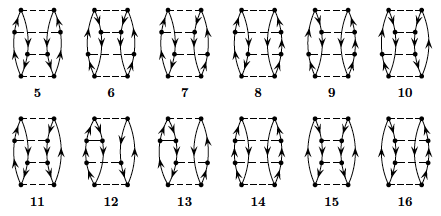
\includegraphics[width=0.6\linewidth]{fig-proj/fourthorder2p2h.png}}
  \caption{
  Two-particle-two-hole excitations to fourth order. \label{fig:fourthorder2p2h}
  }
\end{figure}
%\clearpage % flush figures fig:fourthorder2p2h



\begin{figure}[t]
  \centerline{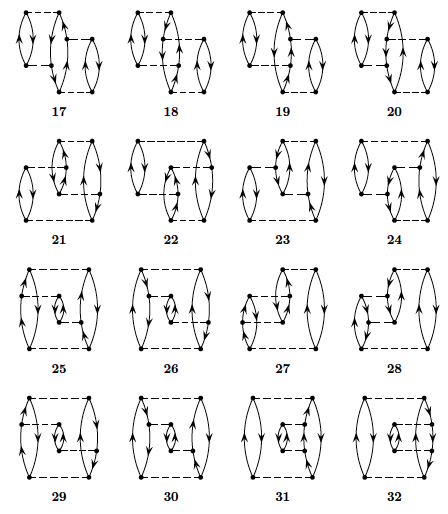
\includegraphics[width=0.6\linewidth]{fig-proj/fourthorder3p3h.png}}
  \caption{
  Three-particle-three-hole excitations to fourth order. \label{fig:fourthorder3p3h}
  }
\end{figure}
%\clearpage % flush figures fig:fourthorder3p3h



\begin{figure}[t]
  \centerline{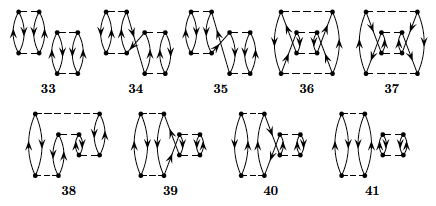
\includegraphics[width=0.6\linewidth]{fig-proj/fourthorder4p4h.png}}
  \caption{
  Four-particle-four-hole excitations to fourth order. \label{fig:fourthorder4p4h}
  }
\end{figure}
%\clearpage % flush figures fig:fourthorder4p4h


Define first linked and unlinked diagrams and explain briefly Goldstone's linked diagram theorem.
Based on the linked diagram theorem and the form of the pairing Hamiltonian, which diagrams will contribute
to fourth order?

Calculate the energy to fourth order with a canonical Hartree-Fock basis for $g\in [-1,1]$ and compare
with the full diagonalization case in exercise b). Discuss the results.


% --- begin solution of exercise ---
\paragraph{Solution.}
To fourth order in the interaction there are several diagrams to consider.
Fortunately, due to the character of the pairing Hamiltonian, several of these contributions are
zero. We limit our discussions also to include the
canonical HF-case only.
All of the diagrams in the canonical case are
shown in figures 3, 4, 5 and 6 above.
Using also the linked diagram theorem, where a
diagram is called unlinked if and only if it has a disconnected part
that is closed, we can eliminate some further  diagrams. Goldstones
linked-diagram theorem states that all unliked diagrams will cancel
against the renormalization terms in Rayleigh-Schroedinger perturbation theory,
meaning that we can define
the energy to each order as a sum of linked diagrams
only. We can then disregard diagram 33 and 41.

Let us now go through all the diagrams and find those that vanish due
to having broken pairs, i.e., the diagrams that vanish due to our
specific interaction. Take for example diagram 1, which vanishes due
to having a term $\langle ab\vert \hat{v} \vert ci\rangle$. From this
argument, we see that all four diagrams from figure 3 vanish. Similar
arguments shows that most diagrams in figure 4 also dissapear. Going
through all the diagrams, we see that 5, 6, 14 and 15 are the ones
that do not vanish in figure 4. For figure 5 we actually see that all
diagrams vanish again. For figure 6 we already found that 33 and 41
vanished due to being unlinked---the rest contribute to the perturbative expansion of the
energy.
The diagrams of figures 3 and 5 vanish since they involve $1p1h$ and $3p3h$ excitations, respectively.

The expressions for these diagrams can easily be written in terms of a
simple Python program. Note however that for every diagram we do
actually perform loops over every single-particle state. As we will
see later, this is extremely inefficient from a computational point
of view. In our discussions of the projects below, we will rewrite the
computations of most diagrams in terms of efficient matrix-matrix
multiplications or matrix-vector multiplications.  The following
Python program gives us the final results for perturbation theory to fourth
order in the interaction. The resulting figures include also plots of the relative error in the
correlation energy. That is, we compare the computed correlation in
perturbation theory with the result from the exact diagonalization discussed above.

\bpypro
from sympy import *
from pylab import *

below_fermi = (0,1,2,3)
above_fermi = (4,5,6,7)

states = [(1,1),(1,-1),(2,1),(2,-1),(3,1),(3,-1),(4,1),(4,-1)]
N = 8
g = Symbol('g')



def h0(p,q):
	if p == q:
		p1, s1 = states[p]
		return (p1 - 1)
	else:
		return 0

def f(p,q):
	if p == q:
		return 0

	s = h0(p,q)
	for i in below_fermi:
		s += assym(p,i,q,i)
	return s


def assym(p,q,r,s):
	p1, s1 = states[p]
	p2, s2 = states[q]
	p3, s3 = states[r]
	p4, s4 = states[s]

	if p1 != p2 or p3 != p4:
		return 0
	if s1 == s2 or s3 == s4:
		return 0
	if s1 == s3 and s2 == s4:
		return -g/2.
	if s1 == s4 and s2 == s3:
		return g/2.

def eps(holes, particles):
	E = 0
	for h in holes:
		p, s = states[h]
		E += (p-1)
	for p in particles:
		p, s = states[p]
		E -= (p-1)
	return E


# Diagram 3
# s = 0
# for a in above_fermi:
# 	for b in above_fermi:
# 		for c in above_fermi:
# 			for i in below_fermi:
# 				for j in below_fermi:
# 					for k in below_fermi:
# 						s += assym(i,j,a,b)*assym(a,c,j,k)*assym(b,k,c,i)/eps((i,j),(a,b))/eps((k,j),(a,c))
# print s


# ga = linspace(-1,1,101)
# corr2 = []
# corr3 = []
# corrx = []


# Diagram 1
s1 = 0
for a in above_fermi:
	for b in above_fermi:
		for i in below_fermi:
			for j in below_fermi:
				s1 += 0.25*assym(a,b,i,j)*assym(i,j,a,b)/eps((i,j),(a,b))

# Diagram 4
s4 = 0
for a in above_fermi:
	for b in above_fermi:
		for c in above_fermi:
			for d in above_fermi:
				for i in below_fermi:
					for j in below_fermi:
						s4 += 0.125*assym(i,j,a,b)*assym(a,b,c,d)*assym(c,d,i,j)/eps((i,j),(a,b))/eps((i,j),(c,d))

# Diagram 5
s5 = 0
for a in above_fermi:
	for b in above_fermi:
		for i in below_fermi:
			for j in below_fermi:
				for k in below_fermi:
					for l in below_fermi:
						s5 += 0.125*assym(i,j,a,b)*assym(k,l,i,j)*assym(a,b,k,l)/eps((i,j),(a,b))/eps((k,l),(a,b))

# Diagram 8 (simplified)
s8 = 0
for a in above_fermi:
	for b in above_fermi:
		for i in below_fermi:
			for j in below_fermi:
				for k in below_fermi:
					s8 -= 0.5*assym(i,j,a,b)*assym(a,b,i,k)*f(k,j)/eps((i,j),(a,b))/eps((i,k),(a,b))

# Diagram 9 (simplified)
s9 = 0
for a in above_fermi:
	for b in above_fermi:
		for c in above_fermi:
			for i in below_fermi:
				for j in below_fermi:
					s9 += 0.5*assym(i,j,a,b)*assym(a,c,i,j)*f(b,c)/eps((i,j),(a,b))/eps((i,j),(a,c))


print s1
print s4
print s5
print s8
print s9

s_5 =  -0.0291521990740741*g**4
s14 =  -0.0308883101851853*g**4
s34 =  0.0163049768518519*g**4
s36 =  -0.0145760995370371*g**4
s38 =  -0.0201099537037037*g**4
s39 =  0.0176938657407407*g**4

ga = linspace(-1,1,10001)
e1 = []
corr2 = []
corr3 = []
corr4 = []
for g_val in ga:
	H1 = matrix([[2-g_val , -g_val/2.,  -g_val/2., -g_val/2., -g_val/2.,     0],
		        [-g_val/2.,   4-g_val,  -g_val/2., -g_val/2.,    0., -g_val/2.],
		        [-g_val/2., -g_val/2.,    6-g_val,     0, -g_val/2., -g_val/2.],
				[-g_val/2., -g_val/2.,      0,   6-g_val, -g_val/2., -g_val/2.],
				[-g_val/2.,     0,  -g_val/2., -g_val/2.,   8-g_val, -g_val/2.],
				[0    , -g_val/2.,  -g_val/2., -g_val/2., -g_val/2.,  10-g_val]])

	u1, v1 = linalg.eig(H1)
	e1.append(min(u1))

	corr2.append((s1).subs(g,g_val))
	corr3.append((s1+s4+s5).subs(g,g_val))
	corr4.append((s1+s4+s5+2*s_5+2*s14+2*s34+2*s36+s38+2*s39).subs(g,g_val))

exact = e1 - (2-ga)

plot(ga, exact, linewidth=2.0)
plot(ga, corr2, linewidth=2.0)
plot(ga, corr3, linewidth=2.0)
plot(ga, corr4, linewidth=2.0)
xlabel(r'Interaction strength, $g$', fontsize=16)
ylabel(r'Correlation energy', fontsize=16)
axis([-1,1,-0.5,0.05])
grid()
legend(["Exact", "2. order MPBT", "3. order MPBT", "4. order MPBT"], 'lower left')
savefig("perturbationtheory.pdf")
show()
error1 = zeros(len(exact))
error2 = zeros(len(exact))
error3 = zeros(len(exact))

for i in range(len(exact)):
	error1[i] = abs(float(exact[i]-corr2[i]))
	error2[i] = abs(float(exact[i]-corr3[i]))
	error3[i] = abs(float(exact[i]-corr4[i]))

error1 = array(error1)
error2 = array(error2)
error3 = array(error3)
print type(error1)

plot(ga, log10(error1))
plot(ga, log10(error2))
plot(ga, log10(error3))
xlabel(r"Strength of interaction, $g$", fontsize=16)
ylabel(r"Error, $\log_{\rm 10}({\rm abs}({\rm error})$", fontsize=16)
legend(["2. order MPBT", "3. order MPBT", "4. order MPBT"], 'lower left')
grid()
savefig("logerror.pdf")
show()
\epypro
Running the Python program shows us that
the approximation to both second and third order are very
good when the interaction strength is small and contained in the interval
$g\in[-0.5,0.5]$, but as the
interaction gets stronger the approximation worsens. We also
note that the third-order result is actually worse than the second order result
for larger values of the interaction strength, indicating that there is no guarantee that higher orders
in many-body perturbation theory may reduce the relative error in a systematic way.
This is seen in particular for the results to fourth order. For negative interaction strengths
fourth order gives a better result than second and third order, while for $g>0$ the relative error is
worse.
We note also the non-variational character of many-body perturbation theory, with results at different undershooting the true ground state correlation energy.

% --- end solution of exercise ---

\end{doconceexercise}
% --- end exercise ---




% --- begin exercise ---
\begin{doconceexercise}
\refstepcounter{doconceexercisecounter}

\subsection*{Project \thedoconceexercisecounter: Coupled cluster calculations with doubles excitations only for the pairing model}


This project serves as a continuation
of the pairing model with the aim being to solve the same problem but
now by developing a program that implements the coupled cluster method
with double excitations only. In doing so you will find it convenient
to write classes which define the single-particle basis and the
Hamiltonian. Your functions that solve the coupled cluster equations
will then just need to set up variables which point to interaction
elements and single-particle states with their pertinent quantum
numbers. Use for example the setup discussed in the FCI lectures for
the pairing model.


\subex{a)}
Explain why no single excitations are involved in this model.

\subex{b)}
Set up the coupled cluster equations for doubles excitations and convince yourself about their
meaning and correctness.

\subex{c)}
Write a class which holds
single-particle data like specific quantum numbers, single-particle
Hamiltonian etc. Write also a class which sets up and stores two-body
matrix elements defined by the single-particle states.  Write
thereafter functions/classes which implement the coupled cluster
method with doubles only.

\subex{d)}
Compare your results with
those from the exact diagonalization with and without the $4p4h$
excitation. Compare also your results to perturbation theory at
different orders, in particular to second order. Discuss your results.
If other students are solving the same problem using Green's function
theory, you can also compare your results with those obtained from
Green's function theory. The aim is to finalize this part during the
first week. The codes you will develop can be used as a starting point
for the second part of the project.

\end{doconceexercise}
% --- end exercise ---




% --- begin exercise ---
\begin{doconceexercise}
\refstepcounter{doconceexercisecounter}

\subsection*{Project \thedoconceexercisecounter: Green's function calculations with a second order self-energy for the pairing model}


This project serves as a continuation of the pairing model with the aim being to solve the same problem but now by developing a program that implements the self-consistent Green's function method with a second order self energy. This is what is called the ADC(2) approximation scheme. In doing so you will find it convenient to write classes which define the single-particle basis and the Hamiltonian. One more, important, class will be needed to store the one-body propagator. Your functions that solve the ADC(3) will then just need to set up variables which point to interaction elements, single-particle states and Dyson states with their pertinent quantum numbers. Use for example the setup discussed in the FCI lectures for the pairing model.


\subex{a)}
Write the diagrams for the self-energy at first and second order, using the Lehman representation for the latter and HF reference state. Write the first order diagrams also in terms of a fully dressed propagator.

\subex{b)}
Set up the Dyson-ADC(2) equations and convince yourself about their meaning and correctness.

\subex{c)}
Write a class that holds the one-body propagator in Lehman representation. In this, the Dyson orbits (or overlap functions) are expanded in terms of the basis exactly as for the HF equations above. However, you will need to handle
a much larger number of orbits and their respective energies. You will also need to store particle and hole orbits separately.
 Using the results of your HF calculations above, build a simple HF propagator. This will be your reference state.

\subex{d)}
Write a class which holds single-particle data like specific quantum numbers, single-particle Hamiltonian etc. Write also a class which sets up and stores two-body matrix elements defined by the single-particle states.

\subex{e)}
Use the above classes to solve the ADC(2) euqatoions in the following three steps:
\begin{itemize}
 \item write the ADC(2) Dyson matrix

 \item diagonalise it (with a Lapack or an eigensolver of your choice)

 \item normalize the eigenvalues, separate them in hole and particle states, and store them in a new propagator object.
\end{itemize}

\noindent
\subex{f)}
Now you can use your ADC(2) code to have some fun:
\begin{itemize}
  \item Plot the spectral functions for the HF (reference) propagator and the final (dressed) result. Compare them. This is the most fun part.  otherwise why should you write a SCGF code for?

  \item Use your solution (the dressed propagator) to recalculate the first order diagram and and implement a partial
     self-consistency loop. See what changes.

  \item Use the Koltun sum rule to calculate the binding energy and compare your results with those from the exact diagonalization with and without the 4p4h excitation. Compare also your results to perturbation theory at different orders, in particular to second order. Discuss your results. If other students are solving the same problem using CCD theory, you can also compare your results with theirs.

  \item How do your results change by increasing the coupling $g$? When is ADC(2)  breaking down for this particular model?
\end{itemize}

\noindent
 The aim is to finalize this part, up to point e), during the first week. The codes you will develop can be used as a starting point for the second part of the project. In the second part we will focus on infinite matter.


\end{doconceexercise}
% --- end exercise ---




% --- begin exercise ---
\begin{doconceexercise}
\refstepcounter{doconceexercisecounter}

\subsection*{Project \thedoconceexercisecounter: Coupled cluster calculations with doubles excitations only for infinite nuclear matter}


This project forms one possible final path for the remaining two weeks. It can also be extended in order to define the final project.  You should be able to use the program you developed in connection with the
solution of the pairing model.


\subex{a)}
Explain why we don't have single excitations in infinite matter.

\subex{b)}
Set up the relavent quantum numbers for a cartesian basis with plane waves in three dimensions. Make the according changes to the code you developed in connection with the pairing model. Implement periodic boundary conditions.

\subex{c)}
Replace the two-body interaction from the pairing model with the Minnesota potential model discussed during the \href{{https://github.com/NuclearTalent/Course2ManyBodyMethods/blob/master/doc/pub/cc/pdf/Lectures1-2_TALENT_NuclearMatter_GH.pdf}}{lectures}.

\subex{d)}
Use the program you developed in connection with the pairing model to perform coupled cluster calculations in infinite matter with doubles excitations.
Perform coupled cluster calculations for infinite nuclear matter with the Minnesota interaction for different particle numbers (to be inserted later).
Limit yourself to two-particle and two-hole intermediate excitations only.

\subex{e)}
Compare the two-particle only excitations with a finite number of particles with results obtained with Brueckner-Hartree-Fock calculations in the thermodynamic limit. Comment your results

\subex{f)}
The final challenge is to include particle-hole excitations and
compare the results with those from Diffusion Monte Carlo calculations
discussed during the \href{{https://github.com/NuclearTalent/Course2ManyBodyMethods/blob/master/doc/pub/cc/pdf/Lectures1-2_TALENT_NuclearMatter_GH.pdf}}{lectures}.
This part can be included in the final project.


\end{doconceexercise}
% --- end exercise ---




% --- begin exercise ---
\begin{doconceexercise}
\refstepcounter{doconceexercisecounter}

\subsection*{Project \thedoconceexercisecounter: Green's function calculations for finite nuclei and infinite nuclear matter}


The hard work in learning how to deal with SCGF was done in Project 2. Now, we make it fancy and extend it to some more real systems rather than a simple pairing model. This can be done very similarly either for finite nuclei or for infinite nuclear matter. However, you should choose only one this two paths and focus only on that: it is already a lot of work doing one. We will do this at the ADC(2) level and toward the end of the project we will consider an extended version of it to make useful comparison with the Brueckner-HF and CCD calculations done by others.

Either of the two path of this project forms one possible final path for the remaining two weeks. It can also be extended in order to define the final project. You should be able to use the program you developed in connection with the solution of the pairing model.


\subex{a)}
Explain why we don't have single excitations in infinite matter.

\subex{b)}
Set up the relavent quantum numbers for your problem:
\begin{enumerate}
 \item For FN:  use and harmonic oscillator basis in m-scheme

 \item for INM: use a cartesian basis with plane waves in three dimensions and implement periodic boundary conditions.
\end{enumerate}

\noindent
In both cases, make the according changes to the code you developed in connection with the pairing model.

\subex{c)}
Replace the two-body interaction from the pairing model with the Minnesota potential model discussed during the lectures (functions for matrix elements in harmonic oscillator basis will be provided).

\subex{d)}
Use the program you developed in connection with the pairing model to perform SCGF calculations at second order. Perform calculations with the Minnesota interaction as follows:

\begin{enumerate}
 \item for finite nuclei chose closed shell systems (He4, C12, O16)
\end{enumerate}

\noindent
  ofor infinite nuclear matter chose different particle numbers (to be inserted later).

At this point, limit yourself to the ADC(2) scheme only.

\subex{e)}
Add the two-particle interactions to the 2p1h sector of the Dyson-ADC(2) matrix and suppress the 2h1p sector: this
should lead you to an approximation equivalent to the Brueckner-Hartree-Fock scheme. Compare your results obtained with
those obetain in CCD with only twp-particle intermediate excitations. If you are doing infinite matter, compare to the  Brueckner-Hartree-Fock calculations in the thermodynamic limit (from project 6). Comment your results.

\subex{f)}
The final challenge is to keep both the 2p1h and the 2h1p sectors and fill the ADC(n) matrix with all the two-particle, the two-hole, and the particle-hole interactions.  This last change results in the so called 'Extended ADC(2)' approximation scheme. Investigate the effects that pp, hh and ph correlations.
This part can be included in the final project. And if you already got all the way to point e), this last part should be a relatively easy improvement to make!

\subex{g)}
Are you felling particularly ambitious? One can further modify the code by adding the missing 3rd order terms to the couplings between the single particle sector and the 2p1h/2h1p sectors. This will give you a full blown ADC(3) calculation. Study the effects of this last change on the energy of the main quasiparticle peaks.  chemist need this to obtain correct ionization potentials and affinities.

\end{doconceexercise}
% --- end exercise ---




% --- begin exercise ---
\begin{doconceexercise}
\refstepcounter{doconceexercisecounter}

\subsection*{Project \thedoconceexercisecounter: Brueckner-Hartree-Fock calculations for infinite nuclear and neutron matter}



\subex{a)}
We will use  the simple Minnesota model discussed during the \href{{https://github.com/NuclearTalent/Course2ManyBodyMethods/blob/master/doc/pub/cc/pdf/Lectures1-2_TALENT_NuclearMatter_GH.pdf}}{lectures}. This will allow us to make detailed comparisons  with the Coupled cluster and the Green's function calculations. The first part deals with setting up the real and imaginary part of $T$-matrix in free space using a partial wave decomposition. You will need to define integration points and weights in momentum space and treat properly the poles which arise. With a working program, compute the relevant phase shifts. Extract also the scattering lengths for $s$ waves (orbital momentum $l=0$).


% --- begin solution of exercise ---
\paragraph{Solution.}
For scattering states, the energy is positive, $E>0$.
The Lippman-Schwinger equation (a rewrite of the Schroedinger equation)
is an integral equation
where we have to deal with the amplitude
$R(k,k')$ (reaction matrix, which is the real part of  the full
complex $T$-matrix)
defined through the integral equation for one partial wave (no coupled-channels)
\begin{equation}
    R_l(k,k') = V_l(k,k') +\frac{2}{\pi}{\cal P}
                \int_0^{\infty}dqq^2V_l(k,q)\frac{1}{E-q^2/m}R_l(q,k').
   \label{eq:ls1}
\end{equation}
For negative energies (bound states) and intermediate states scattering states blocked
by  occupied states below the Fermi level.

The symbol ${\cal P}$ indicates that Cauchy's principal-value prescription
is used in order to avoid the singularity arising from the zero of the denominator.


The total kinetic energy of the two
incoming particles in the center-of-mass system
is
\[
    E=\frac{k_0^2}{m_n}.
\]

The matrix $R_l(k,k')$ relates to the
the  phase shifts through its diagonal elements as
\begin{equation}
     R_l(k_0,k_0)=-\frac{tan\delta_l}{mk_0}.
     \label{eq:shifts}
\end{equation}
In order to solve the Lippman-Schwinger equation
in momentum space, we need first to write
a function which sets up the mesh points.
We need to do that since we are going to approximate an integral
through
\[
   \int_a^bf(x)dx\approx\sum_{i=1}^Nw_if(x_i),
\]
where we have fixed $N$ lattice points through the corresponding weights
$w_i$ and points $x_i$. Typically obtained via methods like Gaussian quadrature.

If you use Gauss-Legendre the points are determined for the interval $x_i\in [-1,1]$
You map these points over to the limits in your integral. You can then
use the following mapping
\[
  k_i=const\times tan\left\{\frac{\pi}{4}(1+x_i)\right\},
\]
and
\[
   \omega_i= const\frac{\pi}{4}\frac{w_i}{cos^2\left(\frac{\pi}{4}(1+x_i)\right)}.
\]
If you choose units fm$^{-1}$ for $k$, set $const=1$. If you choose to work
with MeV, set $const\sim 200$ ($\hbar c=197$ MeVfm).

The principal value integral is rather tricky
to evaluate numerically, mainly since computers have limited
precision. We will here use a subtraction trick often used
when dealing with singular integrals in numerical calculations.
We introduce first the calculus relation
\[
  \int_{-\infty}^{\infty} \frac{dk}{k-k_0} =0.
\]
It means that the curve $1/(k-k_0)$ has equal and opposite
areas on both sides of the singular point $k_0$. If we break
the integral into one over positive $k$ and one over
negative $k$, a change of variable $k\rightarrow -k$
allows us to rewrite the last equation as
\[
  \int_{0}^{\infty} \frac{dk}{k^2-k_0^2} =0.
\]

We can then express a principal values integral
as
\begin{equation}
  {\cal P}\int_{0}^{\infty} \frac{f(k)dk}{k^2-k_0^2} =
  \int_{0}^{\infty} \frac{(f(k)-f(k_0))dk}{k^2-k_0^2},
   \label{eq:trick}
\end{equation}
where the right-hand side is no longer singular at
$k=k_0$, it is proportional to the derivative $df/dk$,
and can be evaluated numerically as any other integral.


We can then use this trick to obtain
\begin{equation}
    R(k,k') = V(k,k') +\frac{2}{\pi}
                \int_0^{\infty}dq
                \frac{q^2V(k,q)R(q,k')-k_0^2V(k,k_0)R(k_0,k')  }
                     {(k_0^2-q^2)/m}.
   \label{eq:ls2}
\end{equation}
This is the equation to solve numerically in order
to calculate the phase shifts. We are interested in obtaining
$R(k_0,k_0)$.

How do we proceed?

Using the mesh points $k_j$ and the weights $\omega_j$, we reach
\[
          R(k,k') = V(k,k') +\frac{2}{\pi}
          \sum_{j=1}^N\frac{\omega_jk_j^2V(k,k_j)R(k_j,k')}
                           {(k_0^2-k_j^2)/m}
           -\frac{2}{\pi}k_0^2V(k,k_0)R(k_0,k')
          \sum_{n=1}^N\frac{\omega_n}
                           {(k_0^2-k_n^2)/m}.
\]
This equation contains now the unknowns $R(k_i,k_j)$
(with dimension $N\times N$) and $R(k_0,k_0)$.

We can turn it into an equation
with dimension $(N+1)\times (N+1)$ with  a mesh
which contains the original mesh points $k_j$ for $j=1,N$
and the point which corresponds to the energy $k_0$.
Consider the latter as the 'observable' point.
The mesh points become then $k_j$ for $j=1,n$ and
$k_{N+1}=k_0$.

With these new mesh points we define the matrix
\begin{equation}
      A_{i,j}=\delta_{i,j}-V(k_i,k_j)u_j,
      \label{eq:aeq}
\end{equation}
where $\delta$ is the Kronecker $\delta$
and
\[
     u_j=\frac{2}{\pi}\frac{\omega_jk_j^2}{(k_0^2-k_j^2)/m}\hspace{1cm} j=1,N
\]
and
\[
     u_{N+1}=-\frac{2}{\pi}\sum_{j=1}^N\frac{k_0^2\omega_j}{(k_0^2-k_j^2)/m}.
\]
The first task is then to
set up the matrix $A$ for a given $k_0$. This is an
$(N+1)\times (N+1)$ matrix. It can be convenient
to have an outer loop which runs over the chosen
observable values for the energy $k_0^2/m$.
\emph{Note that all mesh points $k_j$ for $j=1,N$ must be different from $k_0$. Note also that $V(k_i,k_j)$ is an $(N+1)\times (N+1)$ matrix}.

With the matrix $A$ we can rewrite the problem as a matrix problem of dimension $(N+1)\times (N+1)$.
All matrices $R$, $A$ and $V$ have this dimension and we get
\[
    A_{i,l}R_{l,j}=V_{i,j},
\]
or just
\[
    AR=V.
\]

Since you already have defined $A$ and $V$
(these are stored as $(N+1)\times (N+1)$ matrices)
The final equation involves only the unknown
$R$. We obtain it by matrix inversion, i.e.,
\begin{equation}
    R=A^{-1}V.
    \label{eq:final2}
\end{equation}
Thus, to obtain $R$, you will need to set up the matrices
$A$ and $V$ and invert the matrix $A$.
With the inverse $A^{-1}$, perform
a matrix multiplication with $V$ results in $R$.

With $R$ you can then evaluate the phase shifts
by noting that
\[
      R(k_{N+1},k_{N+1})=R(k_0,k_0)=-\frac{tan\delta}{mk_0},
\]
where $\delta$ are the phase shifts.

% --- end solution of exercise ---

\subex{b)}
Our next step consists in modifying the above program in order to include medium effects.
Rewrite the $T$-matrix program by introducing a so-called angle-average Pauli operator
and corresponding energy denominators. This results in the so-called $G$-matrix.
Allow for the inclusion of single-particle self-energy contributions in the $G$-matrix energy denominators. Compute both the real and imaginary parts of the $G$-matrix and set up the self-consistency problem and compute the ground state energy per particle in the thermodynamical limit.

Compare your results with those obtained with Coupled Cluster theory
and Green's function theory with a cartesian basis


\subex{c)}
In the final part of this project we are going to extend the formalism to finite temperature.
Use the normalization condition of the density from the Fermi-Dirac momentum distribution
to calculate the chemical potential in the medium. Compute thereafter the equation of state
as function of temperature and discuss thermodynamical self-consistency requirements.

\end{doconceexercise}
% --- end exercise ---


% ------------------- end of main content ---------------


% #ifdef PREAMBLE
\printindex

\end{document}
% #endif

